\documentclass[10pt]{article}

\usepackage{fullpage}
\usepackage{color}
\usepackage[table]{xcolor}
\usepackage{hyperref}
\usepackage{graphicx}

%%%%%%%%%%%%%%%%
% Miscellaneous
%%%%%%%%%%%%%%%%

\definecolor{primary}{rgb}{0,0,.50}
%\definecolor{primary}{rgb}{0,0,0}
\definecolor{secondary}{rgb}{.7,.5,0}
\definecolor{table-primary}{rgb}{1,1,1}
\definecolor{table-secondary}{rgb}{.975,.99,1}

%%%%%%%%%%%%%%%%
% Title Section
%%%%%%%%%%%%%%%%

\title{\color{primary}\texttt{UCSC Plaza \\ Sprint1 Review Report}}
\author{{\color{secondary}\textbf{Team Amlesh the Great}} \\ Kyungmin So (PO), Youngsoo Jang, \\ Hobin Ryu, Seungwoo Lee \\ Amlesh Sivanantham, and James Garbagnati }
\date{Release: American Bobtail (July 16, 2016)}

%%%%%%%%%%%%%%%%%%%%%%
% User-Defined Macros
%%%%%%%%%%%%%%%%%%%%%%

%\ignore = Multiline comments
\newcommand{\ignore}[1]{}

\newcommand{\gobblepagenum}{\thispagestyle{empty}\addtocounter{page}{-1}}

%\fancysec{Section title}{Label} = Fancy, colored and labelled section
% Basically just to make it easier to change the format of the whole doc
% Commands with an X are non-numbered sections
\newcommand{\fancysec}[2] {{\color{primary}\section{#1} \label{sec:#2}}}
\newcommand{\fancysub}[2] {{\color{primary}\subsection{#1} \label{sec:#2}}}
\newcommand{\fancysubsub}[2] {{\color{primary}\subsubsection{#1} \label{sec:#2}}}

\newcommand{\fancysecX}[2] {{\color{primary}\section*{#1} \label{sec:#2}}}
\newcommand{\fancysubX}[2] {{\color{primary}\subsection*{#1} \label{sec:#2}}}
\newcommand{\fancysubsubX}[2] {{\color{primary}\subsubsection*{#1} \label{sec:#2}}}


% P.S. I'm so fancy, you already know


%%%%%%%%%%%%%%%%%
% Begin Document
%%%%%%%%%%%%%%%%%
\begin{document}

\maketitle
    
\fancysecX{Actions to stop doing}{stop}
     
        \begin{itemize}
            \item 1. Our team should stop doing holding daily scrum meetings. Because we have another class, finishing development until next scrum meeting is hard.
            \item 2. Our korean member should stop using korean in daily scrum meeting. Because our team member can’t understand korean, and it break our team’s harmony.
        \end{itemize}    

\fancysecX{Actions to start doing}{start}
     
        \begin{itemize}
            \item 1. Our team should learn to communicate effectivley and document the code so it is easier to understand for all team members.
            \item 2. We should start accuratley estimating the work level of our tasks.
            \item 3. We should work faster on our task because sprints are of very short duration.
	\end{itemize}

\fancysecX{Actions to keep doing}{keep}
     
        \begin{itemize}
            \item 1. We should maintain a friendly work environment.
	\end{itemize}
%    \fancysubX{Sprint 2}{sprint2}
        
%        \begin{itemize}
%            \item (5) User Story 1: As an event planner, I want to be able to manage my event, so that I can apply certain constraints to the event.
%            \item (3) User Story 2: As an event-goer, I want to be able to send or rescind an application to a specific event, so that the event planner knows whether I plan to attend or not.
%            \item (3) User Story 3: As an event planner, I want to see who applied to my event and be able to accept or decline their application, so that the event goers know if they are allowed to partake or not.
%            \item (5) User Story 4: As an event-goer, I may wish for privacy settings, so that I can ensure that my event-attendance is not seen by the public.
%            \item (8) User Story 5: As an event-goer, I want to be able to search for specific events, so that I may apply to attend the event.
%        \end{itemize}
         
%    \fancysubX{Sprint 3}{sprint3}
     
%        \begin{itemize}
%            \item (5) User Story 1: As an event-goer, I want to see the current and maximum attendance for the event, so that I can ensure there is space for me to attend and that it is not overcrowded. 
%            \item (5) User Story 2: As an event-planner, I want to ensure that my event does not exceed maximum attendance, so that my event is not overcrowded and has enough room for all event-goers.
%            \item (3) User Story 3: As an event-goer, I want to be able to see and submit my own rating for an event, so that I can decide to go to an ongoing event or offer my opinion towards the event.
%            \item (3) User Story 4: As an event planner, I want to get some feedback on my event, so that I can improve the experience of my event.
%            \item (8) User Story 5: As an event-goer, I want to be able to socialize over an event, so that I can share my opinion with friends and other participants.
%            \item (21) User Story 6: As an event-goer, I want to be able to see if my friends are going to a certain event, so that I know which events have my friends in it.
%            \item (13) User Story 7: As an event-goer, I want to receive recommendations on other events tailored to my preference, so that I can see events that I may attend in the future.
%        \end{itemize}


\fancysecX{Work completed/not completed}{completeWork}

	\fancysubX{Work completed}{completed}
		\begin{itemize}
            \item User Story 1
            \item User Story 2
            \item User Story 4
    	\end{itemize}

    \fancysubX{Work not completed}{notCompleted}
		\begin{itemize}
            \item User Story 3
            \item User Story 5
    	\end{itemize}

\fancysecX{Work completion rate}{completeRate}

	\begin{itemize}
            \item Total number of user stories completed during sprint1 : 2 User stories
    \end{itemize}

    \begin{itemize}
            \item Total number of estimated ideal work hours completed during sprint1 : 10 hours
    \end{itemize}

    \begin{itemize}
            \item Total number of days during sprint1 : 6 days
    \end{itemize}


    \begin{figure}[!ht]
  	\caption{Burnup Chart at the end of sprint 1}
  	\centering
    		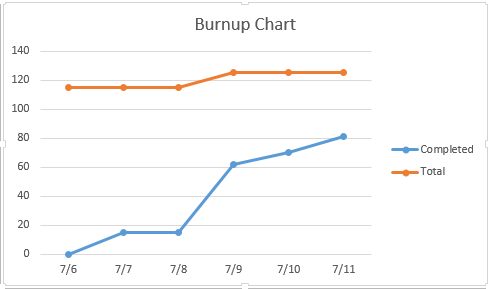
\includegraphics[width=1\textwidth]{Burnupchart1}
    \end{figure}

\vspace{5cm}


\end{document}
